\section{Manuale Utente}
Per confezionare l'applicazione e renderla eseguibile come un'applicazione desktop è 
stato utilizzato Electron: questo framework consente di creare applicazioni 
desktop multi-piattaforma utilizzando tecnologie web come HTML, CSS e JavaScript.

Utilizzando Electron è stato possibile integrare il tutto in un'unica applicazione eseguibile, 
pronta per essere utilizzata dagli utenti senza la necessità di installare ulteriori dipendenze o configurazioni complesse, 
completa e pronta all'uso, che può essere distribuita facilmente tra gli utenti.

In \textit{figura \ref{fig-signin}} è mostrata la pagina di login nel sito, tramite la quale si può accedere inserendo
nome utente e password. 
\begin{figure}[H]
    \centering
    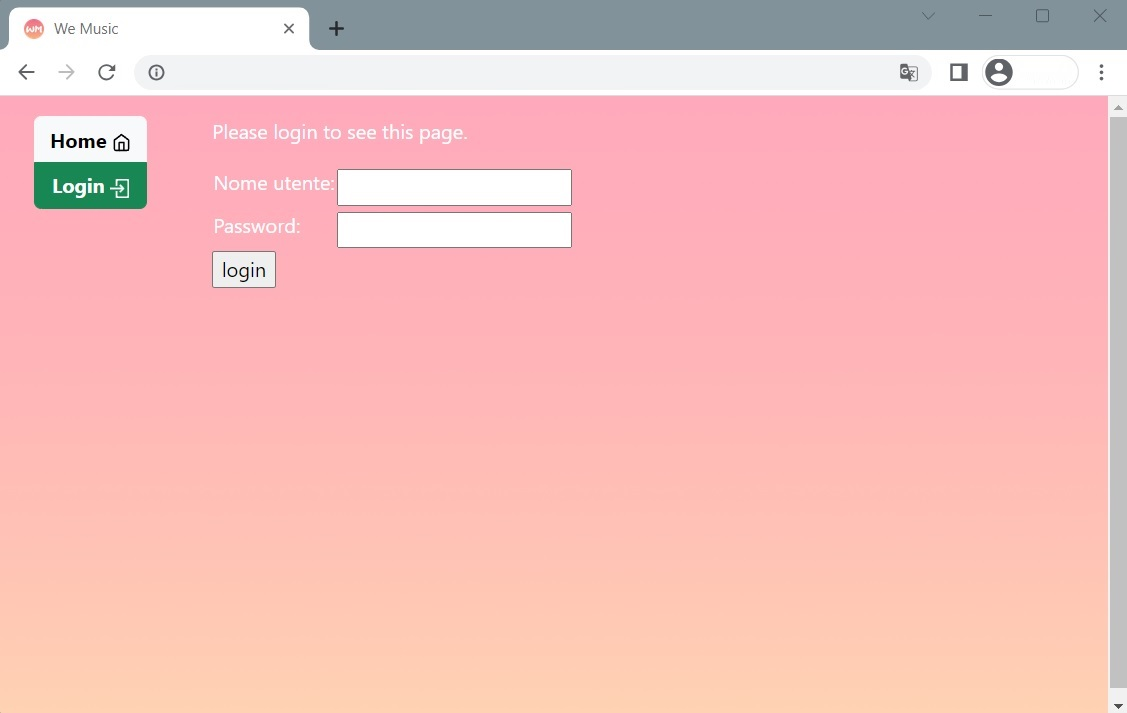
\includegraphics[scale=0.4]{images/login_ver2.jpg}
    \caption{Sign in}
    \label{fig-signin}
\end{figure}
\newpage
Una volta effettuato correttamente l'accesso verrà visualizzata la Homepage del sito, come mostrato 
in \textit{figura \ref{fig-homepage}}. In primo piano è visibile un riepilogo dei brani piaciuti e delle playlist dell'utente,
mentre a sinistra è presente il menu dal quale si può navigare il sito. 
\begin{itemize}
    \item \textbf{Home:} pagina iniziale del sito;
    \item \textbf{Account:} riepilogo infomazioni dell'utente;
    \item \textbf{Discover:} suggerimento brani e amici tramite l'algoritmo;
    \item \textbf{Liked:} riepilogo brani e album piaciuti;
    \item \textbf{Playlist:} riepilogo playlist dell'utente;
    \item \textbf{Social:} pagina di ricerca per aggiungere nuovi amici;
    \item \textbf{Friends:} lista degli amici;
    \item \textbf{Search:} pagina di ricerca per scoprire nuova musica;
\end{itemize} 
\begin{figure}[H]
    \centering
    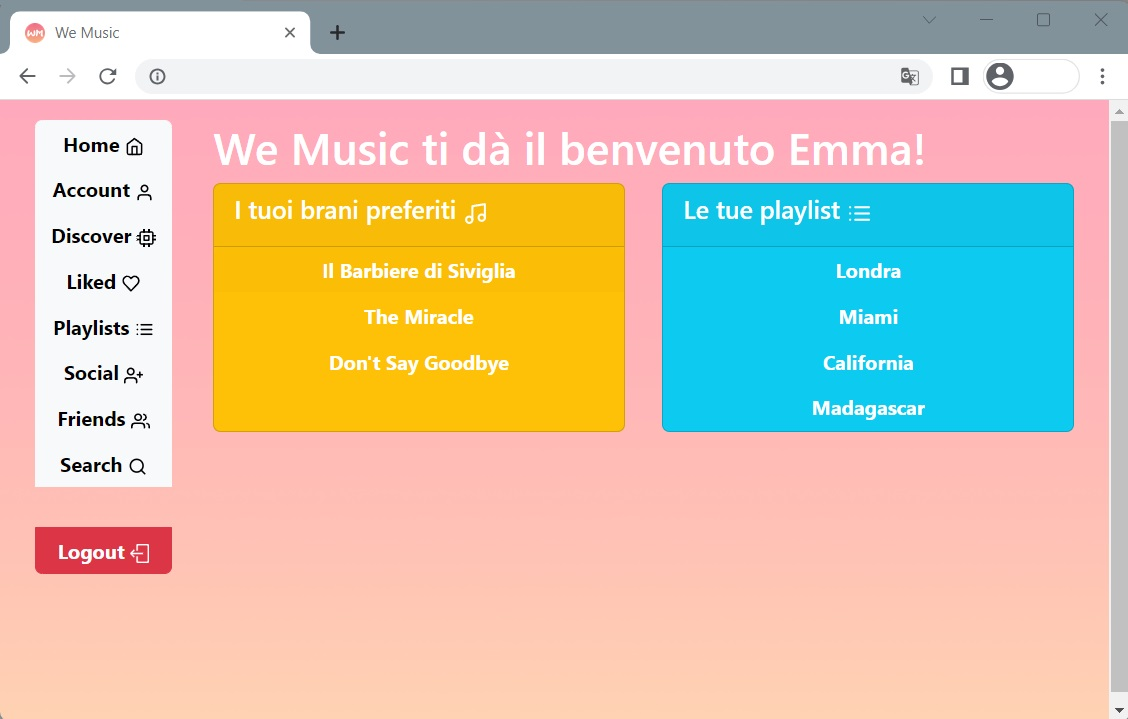
\includegraphics[scale=0.55]{images/homepage_ver2.jpg}
    \caption{Homepage}
    \label{fig-homepage}
\end{figure}
\newpage

\begin{figure}[H]
    \centering
    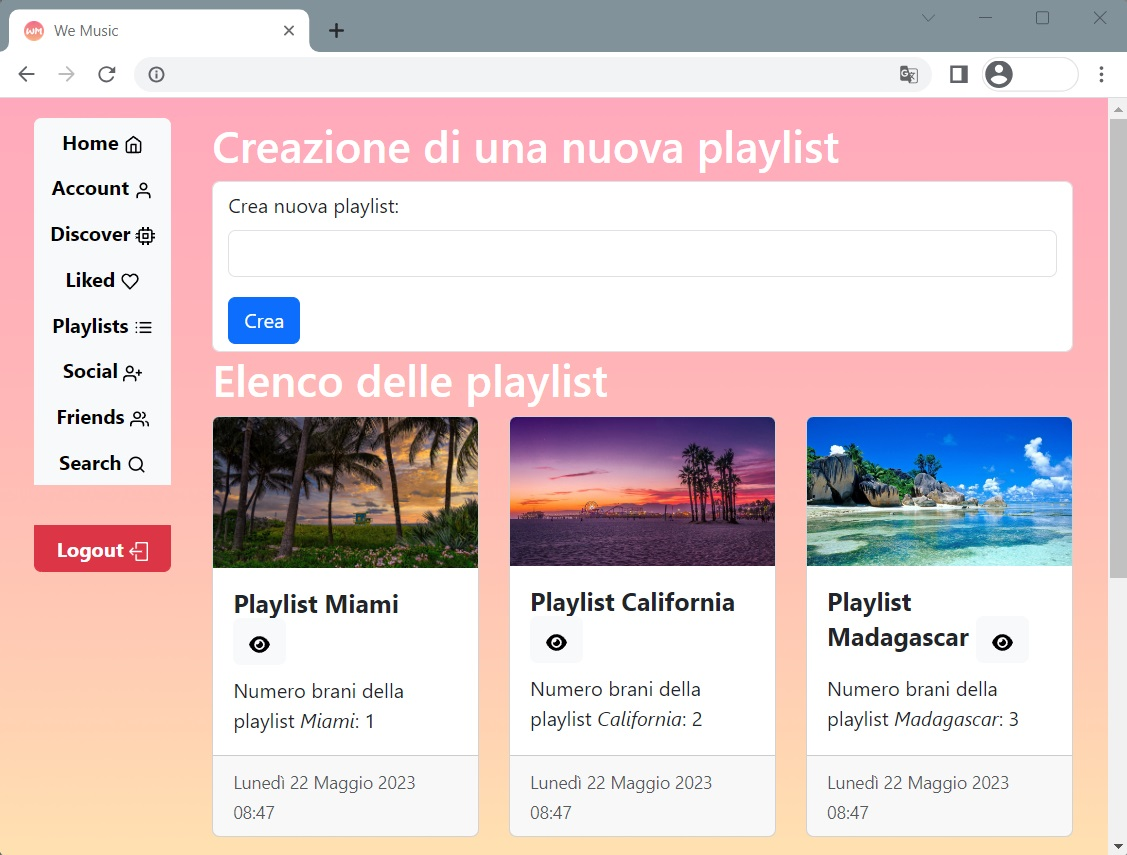
\includegraphics[scale=0.5]{images/playlist_ver2.jpg}
    \caption{Lista playlist}
    \label{fig-playlist}
\end{figure}
\vspace{10pt}
\begin{figure}[H]
    \centering
    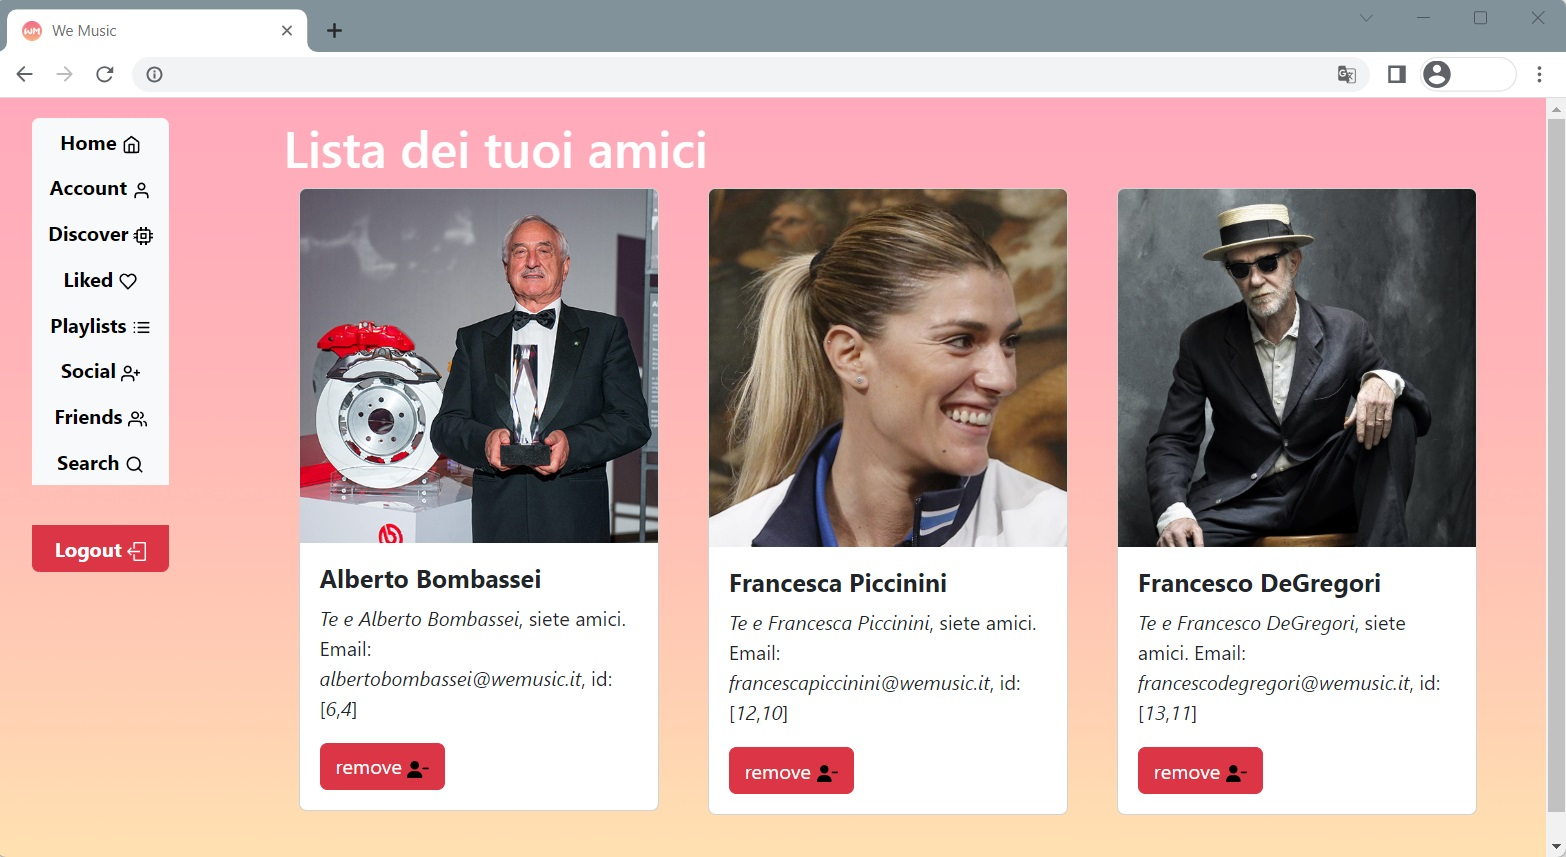
\includegraphics[scale=0.4]{images/amici_ver2.jpg}
    \caption{Lista amici}
    \label{fig-friendslist}
\end{figure}